\documentclass[11pt]{article}
%\documentclass[11pt,dvipdfm]{article}

\usepackage{deauthor}
\usepackage{url}            % simple URL typesetting
\usepackage{graphicx}
\usepackage{times}
\usepackage{fancyvrb}
\usepackage{comment}

% \graphicspath{{authorname/}}

\begin{document}

%\title{MLflow: An Open Platform for Machine Learning Experimentation, Reproducibility and Production}
%\title{MLflow: An Open Platform for the End-to-End Machine Learning Lifecycle}
\title{Accelerating the Machine Learning Lifecycle with {MLflow}}

% The \author macro works with any number of authors. There are two
% commands used to separate the names and addresses of multiple
% authors: \And and \AND.
%
% Using \And between authors leaves it to LaTeX to determine where to
% break the lines. Using \AND forces a line break at that point. So,
% if LaTeX puts 3 of 4 authors names on the first line, and the last
% on the second line, try using \AND instead of \And before the third
% author name.

\author{
  \textbf{Matei Zaharia, Andrew Chen, Aaron Davidson, Ali Ghodsi, Sue Ann Hong, Andy Konwinski,}\\
  \textbf{Siddharth Murching, Tomas Nykodym, Paul Ogilvie, Mani Parkhe, Fen Xie, Corey Zumar} \\
  Databricks Inc.\\
  %% examples of more authors
  %% \And
  %% Coauthor \\
  %% Affiliation \\
  %% Address \\
  %% \texttt{email} \\
  %% \AND
  %% Coauthor \\
  %% Affiliation \\
  %% Address \\
  %% \texttt{email} \\
  %% \And
  %% Coauthor \\
  %% Affiliation \\
  %% Address \\
  %% \texttt{email} \\
  %% \And
  %% Coauthor \\
  %% Affiliation \\
  %% Address \\
  %% \texttt{email} \\
}

\maketitle

\begin{abstract}
Machine learning development creates multiple new challenges that are not present in a traditional software development lifecycle.
These include keeping track of the myriad inputs to an ML application (e.g., data versions, code and tuning parameters), reproducing results, and production deployment.
In this paper, we summarize these challenges from our experience with Databricks customers, and describe MLflow, an open source platform we recently launched to streamline the machine learning lifecycle.
MLflow covers three key challenges: experimentation, reproducibility, and model deployment, using generic APIs that work with any ML library, algorithm and programming language.
The project has a rapidly growing open source community, with over 50 contributors since its launch in June 2018.
\end{abstract}

\section{Introduction}

Machine learning development requires solving new problems that are not part of the standard software development lifecycle.
For example, while traditional software has a well-defined set of product features to be built, ML development tends to revolve around \emph{experimentation}: the ML developer will constantly experiment with new datasets, models, software libraries, tuning parameters, etc.~to optimize a business metric such as model accuracy.
Because model performance depends heavily on the input data and training process, \emph{reproducibility} is paramount throughout ML development.
Finally, in order to have business impact, ML applications need to be \emph{deployed} to production, which means both deploying a model in a way that can be used for inference (e.g., REST serving) and deploying scheduled jobs to regularly update the model.
This is especially challenging when deployment requires collaboration with another team, such as application engineers who are not ML experts.

Based on our conversations with dozens of Databricks customers that use machine learning, these lifecycle problems are a major bottleneck in practice.
Although today's ML libraries provide tools for part of the lifecycle, there are no standard systems and interfaces to manage the full process.
For example, TensorFlow offers a training API and a Serving system~\cite{tfx}, but TensorFlow Serving cannot easily be used for models from another ML library, or from an incompatible version of TensorFlow.
In practice, an organization will need to run models from multiple ML libraries, TensorFlow versions, etc., and has to design its own infrastructure for this task.


Faced with these challenges, many organizations try to ``lock down'' the ML development process to obtain reproducibility and deployability.
Some organizations develop internal guidelines for ML development, such as which libraries one can use that the production team will support.
Others develop internal \emph{ML platforms} (e.g., Facebook's FBLearner~\cite{fblearner}, Uber's Michelangelo~\cite{michelangelo} and Google's TFX~\cite{tfx}): APIs that ML developers must use in order to build deployable models.
Unfortunately, both approaches limit ML developers in the algorithms and libraries they can use, decreasing their ability to experiment, and both create substantial engineering work whenever the ML developers want to use new libraries or models.

%Some organizations ask each ML team to manage its own infrastructure, which is expensive.
%Others try to develop shared \emph{ML platforms} that data scientists must use to build their models (e.g., Facebook's FBLearner~\cite{fblearner} and Uber's Michelangelo~\cite{michelangelo}), but this approach also has challenges, because model developers are limited to the algorithms and libraries supported by the platform and cannot easily experiment with others.

In this paper, we summarize our experience with ML lifecycle challenges at Databricks customers and describe MLflow, an open source ML platform we are developing to address these challenges.
MLflow's key principle is an \emph{open interface} design, where data scientists and engineers can bring their own training code, metrics, and inference logic while benefitting from a structured development process.
%MLflow leverages simple, generic interfaces such as Docker containers and REST APIs to achieve this goal.
For example, a ``model'' saved in MLflow can simply be a Python function (and associated library dependencies) that MLflow then knows how to deploy in various environments (e.g., batch or real-time scoring).
Other MLflow abstractions are likewise based on generic interfaces, such as REST APIs and Docker containers.
Compared to existing ML platforms like FBLearner, Michelangelo and TFX, this open interface design gives users flexibility and control while retaining the benefits of lifecycle management.
%Moreover, MLflow's open source nature enables easily sharing ML work across organizations.
The current version of MLflow provides APIs for experiment tracking, reproducible runs and model packaging and deployment, usable in Python, Java and R.
We describe these APIs and some sample MLflow use cases to show how the system can streamline the machine learning lifecycle.

\section{Challenges in Machine Learning Development}

ML faces many of the challenges in traditional software development, such as testing, code review, monitoring, etc.
In other ways, however, ML applications are different from traditional software, and present new problems.

One of the main differences is that the goal in machine learning is to \emph{optimize} a specific metric, such as prediction accuracy, instead of simply meeting a set of functional requirements.
For example, for a retailer, every 1\% improvement in prediction accuracy for a recommendation engine might lead to millions of dollars in revenue, so the ML team working on this engine will continuously want to improve the model.
This means that ML developers wish to continuously experiment with the latest models, software libraries, etc.,~to improve target metrics.
Beyond this difference in objective, ML applications are more complex to manage because their performance depends on training data, tuning, and concerns such as overfitting that do not occur in other applications.
%This means that reproducibility of these runtime conditions is important.
Finally, ML applications are often developed by teams or individuals with very different expertise, and hand-off between these individuals can be challenging.
For example, a data scientist might be an expert at ML training, and use her skills to create a model, but she might need to pass the model to a software engineer for deployment within an application.
Any errors in this process (e.g., mismatched software versions or data formats) might lead to incorrect results that are hard for a software engineer without ML knowledge to debug.

Based on these requirements in working with ML, we found four challenges to arise repeatedly at ML users:

\vspace{-0.6em}
\paragraph{1. Multitude of tools.} Hundreds of software tools cover each phase of ML development, from data preparation to model training to deployment. However, unlike traditional software development, where teams select \emph{one} tool for each phase, ML developers usually want to try \emph{every} available tool (e.g., algorithm) to see whether it improves results. For example, a team might try multiple preprocessing libraries (e.g., Pandas and Apache Spark) to featurize data; multiple model types (e.g. trees and deep learning); and even multiple frameworks for the same model type (e.g., TensorFlow and PyTorch) to run various models published online by researchers. %This diversity of tools means that ML teams need to use and productionize dozens of libraries.

\vspace{-0.6em}
\paragraph{2. Experiment tracking.} Machine learning results are affected by dozens of configurable parameters, ranging from the input data to hyperparameters and preprocessing code. Whether an individual is working alone or on a team, it is difficult to track which parameters, code, and data went into each experiment to produce a model.

\vspace{-0.6em}
\paragraph{3. Reproducibility.} Without detailed tracking, teams often have trouble getting the same code to work again. For example, a data scientist passing her training code to an engineer for use in production might see problems if the engineer modifies it, and even a user working alone needs to reliably reproduce old results to stay productive. %Even ML researchers frequently experience this problem when trying to reproduce published work.

\vspace{-0.6em}
\paragraph{4. Production deployment.} Moving an application to production can be challenging, both for inference and training. First, there are a plethora of possible inference environments, such as REST serving, batch scoring and mobile applications, but there is no standard way to move models from any library to these diverse environments. Second, the model training pipeline also needs to be reliably converted to a scheduled job, which requires care to reproduce the software environments, parameters, etc.~used in development.
Production deployment is especially challenging because it often requires passing the ML application to a different team with less ML expertise.

~

\vspace{-0.6em}
To address these problems, we believe that ML development processes should be explicitly designed to promote reproducibility, deployability, etc. The challenge is how to do so while leaving maximum flexibility for ML developers to build the best possible model. This led us to the open interface design philosophy for MLflow.

\section{MLflow Overview}

To structure the ML development process while leaving users maximum flexibility, we built MLflow around an \emph{open interface} philosophy: the system should define general interfaces for each abstraction (e.g., a training step, a deployment tool or a model) that allow users to bring their own code or workflows.
For example, many existing ML tools represent models using a serialization format, such as TensorFlow graphs~\cite{abadi2016tensorflow}, ONNX~\cite{onnx} or PMML~\cite{pmml}, when passing them from training to serving. This restricts applications to using specific libraries.
In contrast, in MLflow, a model can be represented simply as a Python function (and library dependency information), so any development tool that knows how to run a Python function can run such a model.
For more specialized deployment tools, a model can also expose other interfaces called ``flavors" (e.g., an ONNX graph) while still remaining viewable as just a Python function.
As another example, MLflow exposes most of its features through REST APIs that can called from any programming language.

More specifically, MLflow provides three components, which can either be used together or separately:

\begin{itemize}
\item \textbf{MLflow Tracking}, which is an API for recording experiment runs, including code used, parameters, input data, metrics, and arbitrary output files. These runs can then be queried through an API or UI.

\item\textbf{MLflow Projects}, a simple format for packaging code into reusable projects. Each project defines its environment (e.g., software libraries required), the code to run, and parameters that can be used to call the project programmatically in a multi-step workflow or in automated tools such as hyperparameter tuners.

\item\textbf{MLflow Models}, a generic format for packaging models (both the code and data required) that can work with diverse deployment tools (e.g., batch and real-time inference). %The goal is to give users of the model (e.g., a production engineer) a consistent interface for working with models built in different tools.
\end{itemize}

%We next sketch these components in turn; full documentation on them is available at \url{mlflow.org}.

\subsection{MLflow Tracking}

MLflow Tracking is an API for logging and querying \emph{experiment runs}, which consist of parameters, code versions, metrics and arbitrary output files called \emph{artifacts}. Users can start/end runs and log metrics, parameters and artifacts using simple API calls, as shown below using MLflow's Python API:

\begin{Verbatim}[frame=single,fontsize=\small,samepage=true]
# Log parameters, which are arbitrary key-value pairs
mlflow.log_param("num_dimensions", 8)
mlflow.log_param("regularization", 0.1)

# Log metrics; each metric can also be updated throughout the run
mlflow.log_metric("accuracy", 0.8)
mlflow.log_metric("r2", 0.4)

# Log artifacts (arbitrary output files)
mlflow.log_artifact("precision_recall.png")
\end{Verbatim}

MLflow Tracking API calls can be inserted anywhere users run code (e.g., standalone applications or Jupyter notebooks running in the cloud). The tracking API logs results to a local directory by default, but it can also be configured to log over the network to a server, allowing teams to share a centralized MLflow tracking server and compare results from multiple developers.

Once users have recorded runs, MLflow allows users to query them through an API or web-based UI (Figure~\ref{fig:tracking-ui}). This UI includes the ability to organize runs into groups called Experiments, search and sort them, and compare groups of runs, enabling users to build a custom leaderboard for each of their ML problems and even compare results across teams. The UI is inspired by experiment visualization tools such as Sacred~\cite{sacred}, ModelDB~\cite{modeldb} and TensorBoard~\cite{tensorboard}, and supports similar visualizations and queries.

\begin{figure}[h]
\centering
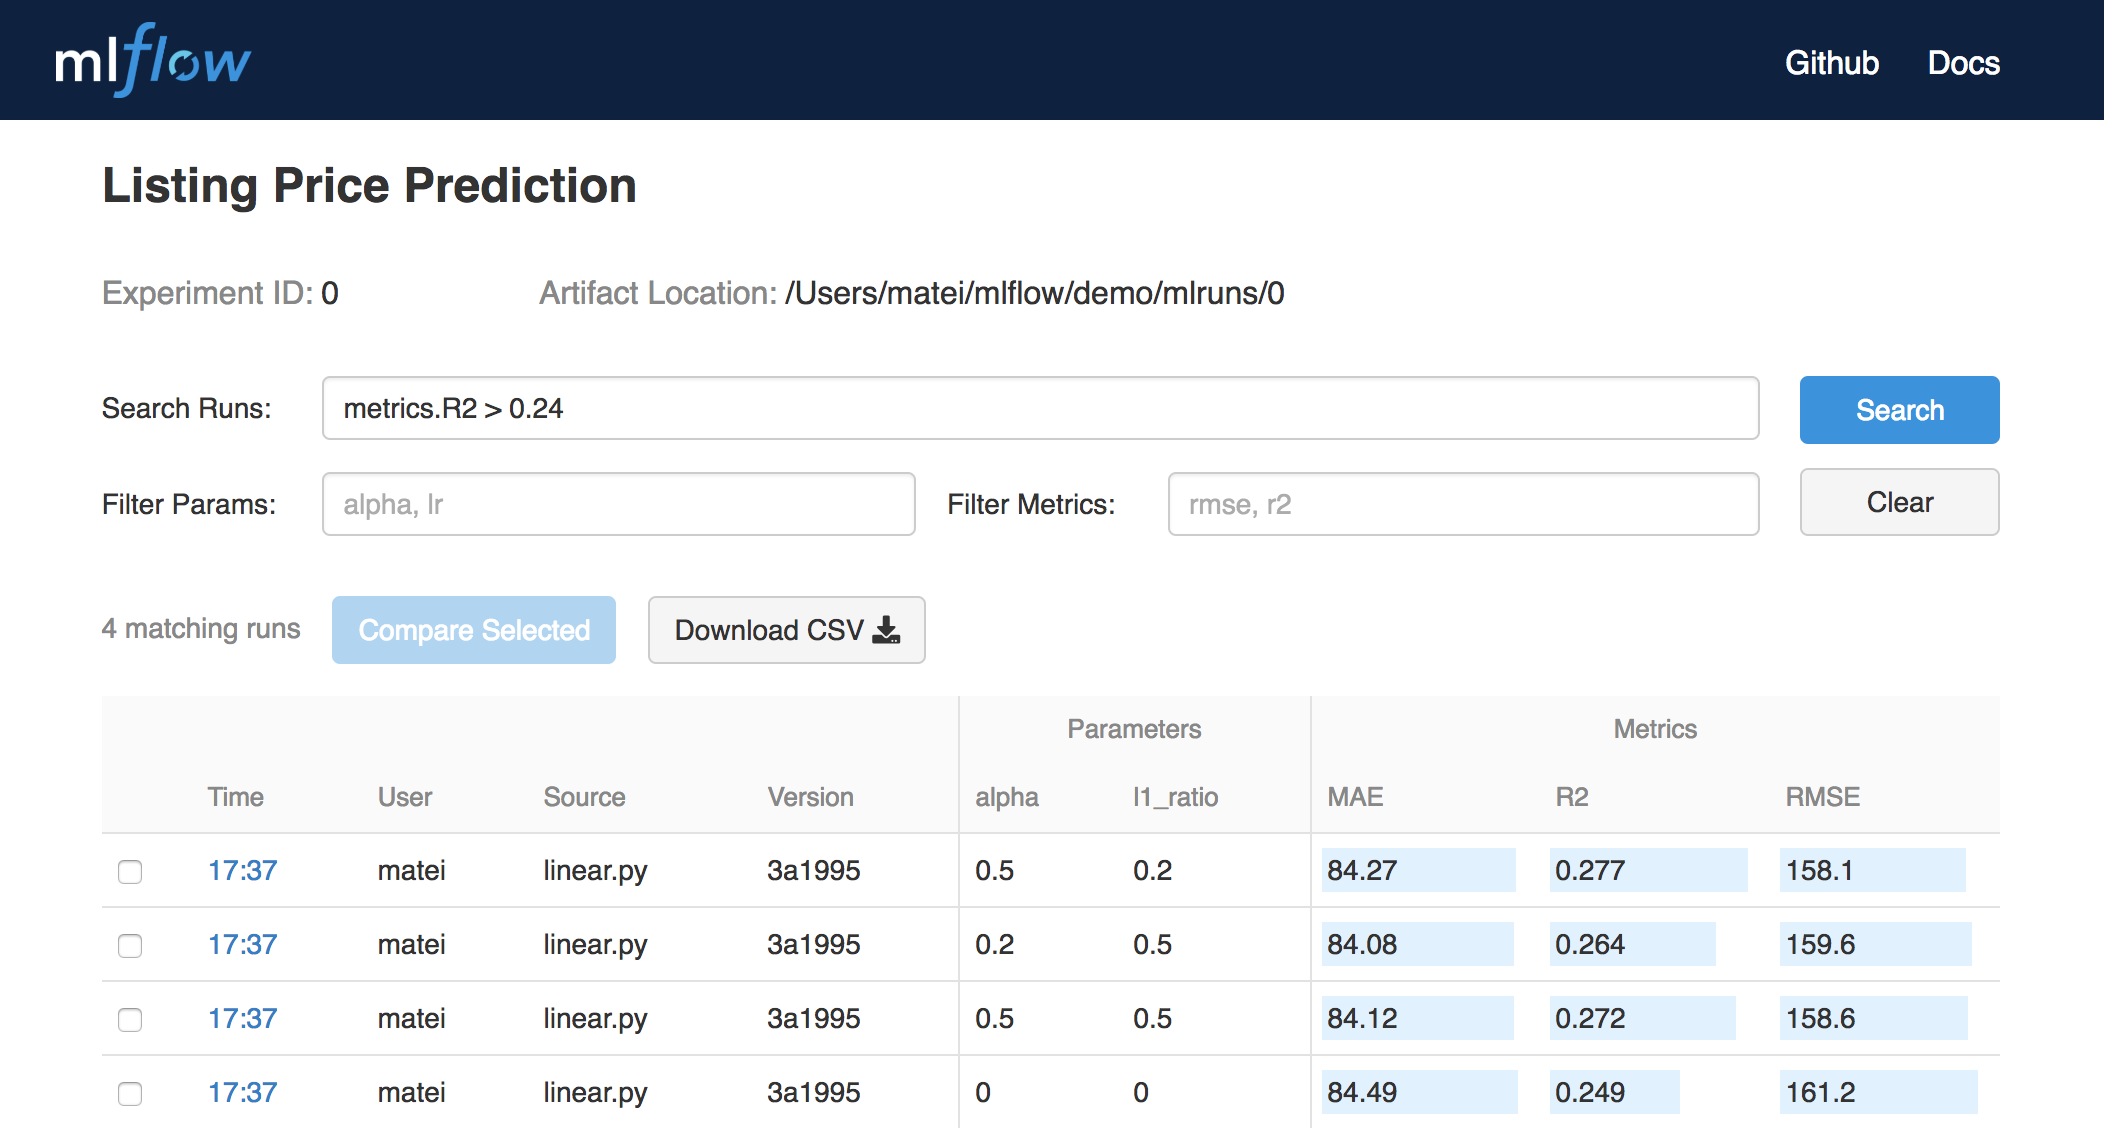
\includegraphics[width=\textwidth]{tracking.png}
\caption{MLflow Tracking UI showing several runs in an experiment. Clicking each run lists its metrics, artifacts and output details and lets the user post comments about the run.}
\label{fig:tracking-ui}
\end{figure}

\subsection{MLflow Projects}

MLflow Projects provide a simple format for packaging reproducible data science code. Each project is simply a directory with code or a Git repository, and uses a descriptor file to specify its dependencies and how to run the code. A MLflow Project is defined by a simple YAML file called MLproject, as shown below:

\begin{Verbatim}[frame=single,fontsize=\small,samepage=true]
name: My Project
conda_env: conda.yaml
entry_points:
  main:
    parameters:
      data_file: path
      alpha: {type: float, default: 0.1}
    command: "python train.py --reg-param {alpha} --data {data_file}"
\end{Verbatim}


Projects can specify their dependencies through a Conda environment or (in an upcoming release) a Docker container specification. A project may also have multiple entry points for invoking runs, with named parameters that downstream users can provide without understanding the internals of the project.

Users can run projects using the \texttt{mlflow run} command line tool, either from local files or a Git repository:

\begin{Verbatim}[frame=single,fontsize=\small,samepage=true]
mlflow run git@github.com:databricks/mlflow-example.git -P alpha=0.5
\end{Verbatim}

Alternatively, projects can be called programmatically using MLflow's API. This can be used to implement multi-step workflows or to pass projects a ``black box'' into automated tools such as hyperparameter search~\cite{hyperopt}.

In either case, MLflow will automatically set up the project's runtime environment and execute it. If the code inside the project uses the MLflow Tracking API, MLflow will also remember the project version executed (that is, the Git commit) and show an \texttt{mlflow run} command to re-execute it in its UI. Finally, MLflow projects can also be submitted to cloud platforms such as Databricks for remote execution.

\subsection{MLflow Models}

MLflow Models are a convention for packaging machine learning models in multiple formats called ``flavors'', allowing diverse tools to understand the model at different levels of abstractions. MLflow also offers a variety of built-in tools to deploy models in its standard favors. For example, the same model can be deployed as a Docker container for REST serving, as an Apache Spark user-defined function (UDF) for batch inference, or into cloud-managed serving platforms like Amazon SageMaker and Azure ML.

Each MLflow Model is simply stored as a directory containing arbitrary files and an MLmodel YAML file that lists the flavors it can be used in and additional metadata about how it was created:

\begin{Verbatim}[frame=single,fontsize=\small,samepage=true]
time_created: 2018-02-21T13:21:34.12
run_id: c4b65fc2c57f4b6d80c6e58a9dcb9f01
flavors:
  sklearn:
    sklearn_version: 0.19.1
    pickled_model: model.pkl
  python_function:
    loader_module: mlflow.sklearn
    pickled_model: model.pkl
\end{Verbatim}

In this example, the model can be used with tools that support either the \texttt{sklearn} or \texttt{python\_function} model flavors. For example, the MLflow SciKit-Learn library knows how to load a \texttt{sklearn} model as a SciKit-Learn Python object, but other deployment tools, such as running the model in a Docker HTTP server, only understand lower-level flavors like \texttt{python\_function}.
In addition, models logged using MLflow Tracking APIs will automatically include a reference to that run's unique ID, letting users discover how they were built.

\section{Example Use Cases}

In this section, we describe three sample MLflow use cases to highlight how users can leverage each component.

\vspace{-0.6em}
\paragraph{Experiment tracking.} A European energy company is using MLflow to track and update hundreds of energy grid models. This team's goal is to build a time series model for every major energy producer (e.g., power plant) and consumer (e.g., factory), monitor these using standard metrics, and combine the predictions to drive business processes such as pricing. Because a single team is responsible for hundreds of models, possibly using different ML libraries, it was important to have a standard development and tracking process. The team has standardized on using Jupyter notebooks for development, MLflow Tracking for metrics, and Databricks jobs for inference.

\vspace{-0.6em}
\paragraph{Reproducible projects.} An online marketplace is using MLflow Projects to package deep learning jobs using Keras and run them in the cloud. Each data scientist develops models locally on his or her laptop using a small dataset, checks them into a Git repository with an MLproject file, and submits remote runs of the project to GPU instances in the cloud for large-scale training or hyperparameter search. Using MLflow Projects makes it easy to create the same software environment in the cloud and share project code between different data scientists.

\vspace{-0.6em}
\paragraph{Model packaging.} The data science team at an e-commerce site is using MLflow Models to package recommendation models for use by application engineers. The technical challenge here was that the recommendation application includes both a standard, ``off-the-shelf'' recommendation model and custom business logic for pre- and post-processing. For example, the application might include custom code to make sure that the recommended items are diverse. This business logic needs to change in sync with the model, and the data science team wants to control both the business logic and the model, without having to submit a patch to the web application each time this logic has to change.
Moreover, the team wants to A/B test distinct models with distinct versions of the processing logic.
The solution was to package both the recommendation model and the custom logic using the \texttt{python\_function} flavor in an MLflow Model, which can then be deployed and tested as a single unit. %This allows production engineers to deploy the recommendation code as they please without the processing logic falling out of sync with the model.

\section{Related Work}

Many software systems aim to simplify ML development.
The closest to our work are the end-to-end ``ML platforms'' at large web companies.
For example, Facebook's FBLearner lets users write reusable workflow steps that run over data in Apache Hive~\cite{fblearner};
Uber's Michelangelo gives users a toolkit of algorithms to choose from that it can automatically train and deploy~\cite{michelangelo}; and Google's TFX provides data preparation and serving tools around TensorFlow~\cite{tfx}.
Anecdotally, these platforms greatly accelerate ML development, showing the benefits of standardizing the ML lifecycle.
However, they generally restrict users to a specific set of algorithms or libraries, so teams are on their own when they step outside these boundaries.
Our goal in MLflow is to let users easily bring their own tools and software in as many steps in the process as possible through our ``open interface'' design.
This includes custom training steps, inference code, and logged parameters and artifacts.

Other systems also tackle specific problems within the ML lifecycle. For example, Sacred~\cite{sacred}, ModelDB~\cite{modeldb} and TensorBoard~\cite{tensorboard} let users track experiments; PMML~\cite{pmml} and ONNX~\cite{onnx} are cross-library model serialization formats; Clipper~\cite{clipper} can deploy arbitrary models as Docker containers; and CDE~\cite{cde}, CodaLab~\cite{codalab}, Binder~\cite{binder} and Repo2Docker~\cite{repo2docker} enable reproducible software runs. MLflow combines these concepts with new ones, such as multi-flavor model packaging, into a unified system design and API.

\section{Conclusion}

For machine learning to have widespread commercial impact, organizations require the same kinds of reliable engineering processes around ML that exist in other engineering disciplines such as software development. In this paper, we have described some of the key challenges that differentiate ML development from traditional software development, such as experimentation, reproducibility, and reliable production deployment. We have also described MLflow, a software platform that can structure the machine learning lifecycle while giving users broad flexibility to use their own ML algorithms, software libraries and development processes.
MLflow is available as open source software at \url{https://www.mlflow.org}.


{\small

\begin{thebibliography}{10}

  \bibitem{abadi2016tensorflow}
  M.~Abadi, P.~Barham, J.~Chen, Z.~Chen, A.~Davis, J.~Dean, M.~Devin,
    S.~Ghemawat, G.~Irving, M.~Isard, et~al.
  \newblock {TensorFlow: A System for Large-Scale Machine Learning}.
  \newblock In {\em OSDI}, volume~16, pages 265--283, 2016.

  \bibitem{tfx}
  D.~Baylor, E.~Breck, H.-T. Cheng, N.~Fiedel, C.~Y. Foo, Z.~Haque, S.~Haykal,
    M.~Ispir, V.~Jain, L.~Koc, C.~Y. Koo, L.~Lew, C.~Mewald, A.~N. Modi,
    N.~Polyzotis, S.~Ramesh, S.~Roy, S.~E. Whang, M.~Wicke, J.~Wilkiewicz,
    X.~Zhang, and M.~Zinkevich.
  \newblock Tfx: A tensorflow-based production-scale machine learning platform.
  \newblock In {\em Proceedings of the 23rd ACM SIGKDD International Conference
    on Knowledge Discovery and Data Mining}, KDD '17, pages 1387--1395, New York,
    NY, USA, 2017. ACM.

  \bibitem{hyperopt}
  J.~Bergstra, B.~Komer, C.~Eliasmith, D.~Yamins, and D.~D. Cox.
  \newblock Hyperopt: a python library for model selection and hyperparameter
    optimization.
  \newblock {\em Computational Science and Discovery}, 8(1):014008, 2015.

  \bibitem{binder}
  {Binder}.
  \newblock \url{https://mybinder.org}, 2018.

  \bibitem{clipper}
  D.~Crankshaw, X.~Wang, G.~Zhou, M.~J. Franklin, J.~E. Gonzalez, and I.~Stoica.
  \newblock Clipper: A low-latency online prediction serving system.
  \newblock In {\em Proceedings of the 14th USENIX Conference on Networked
    Systems Design and Implementation}, NSDI'17, pages 613--627, Berkeley, CA,
    USA, 2017. USENIX Association.

  \bibitem{fblearner}
  J.~Dunn.
  \newblock Introducing {FBLearner Flow}: Facebook’s {AI} backbone.
  \newblock
    \url{https://code.fb.com/core-data/introducing-fblearner-flow-facebook-s-ai-backbone/}.

  \bibitem{repo2docker}
  J.~Forde, T.~Head, C.~Holdgraf, Y.~Panda, G.~Nalvarte, M.~Pacer, F.~Perez,
    B.~Ragan-Kelley, and E.~Sundell.
  \newblock Reproducible research environments with repo2docker.
  \newblock ICML, 07/2018 2018.

  \bibitem{tensorboard}
  Google.
  \newblock Tensorboard: Visualizing learning.
  \newblock \url{https://www.tensorflow.org/guide/summaries_and_tensorboard}.

  \bibitem{pmml}
  A.~Guazzelli, W.-C. Lin, and T.~Jena.
  \newblock {\em PMML in Action: Unleashing the Power of Open Standards for Data
    Mining and Predictive Analytics}.
  \newblock CreateSpace, Paramount, CA, 2nd edition, 2012.

  \bibitem{cde}
  P.~J. Guo.
  \newblock {CDE}: A tool for creating portable experimental software packages.
  \newblock {\em Computing in Science and Engineering}, 14(4):32--35, 2012.

  \bibitem{michelangelo}
  J.~Hermann and M.~D. Balso.
  \newblock Meet {Michelangelo}: Uber’s machine learning platform.
  \newblock \url{https://eng.uber.com/michelangelo/}.

  \bibitem{sacred}
  {K}laus {G}reff, {A}aron {K}lein, {M}artin {C}hovanec, {F}rank {H}utter, and
    {J}\"urgen {S}chmidhuber.
  \newblock {T}he {S}acred {I}nfrastructure for {C}omputational {R}esearch.
  \newblock In {K}aty {H}uff, {D}avid {L}ippa, {D}illon {N}iederhut, and
    M.~{P}acer, editors, {\em {P}roceedings of the 16th {P}ython in {S}cience
    {C}onference}, pages 49 -- 56, 2017.

  \bibitem{codalab}
  P.~Liang et~al.
  \newblock {CodaLab}.
  \newblock \url{https://worksheets.codalab.org}, 2018.

  \bibitem{onnx}
  {ONNX Group}.
  \newblock {ONNX}.
  \newblock \url{https://onnx.ai}.

  \bibitem{modeldb}
  M.~Vartak, H.~Subramanyam, W.-E. Lee, S.~Viswanathan, S.~Husnoo, S.~Madden, and
    M.~Zaharia.
  \newblock Modeldb: A system for machine learning model management.
  \newblock In {\em Proceedings of the Workshop on Human-In-the-Loop Data
    Analytics}, HILDA '16, pages 14:1--14:3, New York, NY, USA, 2016. ACM.

  \end{thebibliography}


}
%\bibliographystyle{abbrv}
%\bibliography{paper}

\end{document}
